\documentclass{ieeeaccess}
\usepackage{cite}
\usepackage{amsmath,amssymb,amsfonts}
\usepackage{graphicx}
\usepackage{textcomp}
\usepackage{booktabs}
\usepackage{bm}
\makeatletter
\AtBeginDocument{\DeclareMathVersion{bold}
\SetSymbolFont{operators}{bold}{T1}{times}{b}{n}
\SetSymbolFont{NewLetters}{bold}{T1}{times}{b}{it}
\SetMathAlphabet{\mathrm}{bold}{T1}{times}{b}{n}
\SetMathAlphabet{\mathit}{bold}{T1}{times}{b}{it}
\SetMathAlphabet{\mathbf}{bold}{T1}{times}{b}{n}
\SetMathAlphabet{\mathtt}{bold}{OT1}{pcr}{b}{n}
\SetSymbolFont{symbols}{bold}{OMS}{cmsy}{b}{n}
\renewcommand\boldmath{\@nomath\boldmath\mathversion{bold}}}
\makeatother
\graphicspath{{../../results/v2/figures/}}
\newcommand{\tabsize}{\footnotesize}

\begin{document}
\history{Date of publication xxxx 00, 0000, date of current version xxxx 00, 0000.}
\doi{10.1109/ACCESS.2026.0000000}

\title{Does Dimensionality Reduction Help Classical Intrusion Detection? Original Features versus PCA and Kernel PCA on a Class-Stratified CIC-IDS2017 Sample}
\author{\uppercase{[AUTHOR NAME 1 - TO BE FILLED]}\authorrefmark{1},
\uppercase{[AUTHOR NAME 2 - TO BE FILLED]}\authorrefmark{2}}

\address[1]{[DEPARTMENT, INSTITUTION, CITY, COUNTRY - TO BE FILLED] (e-mail: [EMAIL - TO BE FILLED])}
\address[2]{[DEPARTMENT, INSTITUTION, CITY, COUNTRY - TO BE FILLED] (e-mail: [EMAIL - TO BE FILLED])}
\tfootnote{[FUNDING / SUPPORT STATEMENT - TO BE FILLED BY THE AUTHORS, OR DELETE THIS FOOTNOTE IF THERE IS NONE]}

\markboth
{Author \headeretal: Dimensionality Reduction for Classical Intrusion Detection}
{Author \headeretal: Dimensionality Reduction for Classical Intrusion Detection}

\corresp{Corresponding author: [NAME - TO BE FILLED] (e-mail: [EMAIL - TO BE FILLED]).}

\begin{abstract}
Kernel principal component analysis is often paired with classical classifiers for network intrusion detection, but gains are usually reported as single-split accuracy without a no-reduction baseline. This study compares the 78 original flow features with principal component analysis and kernel principal component analysis (linear, radial basis function and cosine kernels; 5 to 30 components) across five classifiers. The data are a 6,000-record sample drawn from all eight CIC-IDS2017 files after exact-duplicate removal. The sample is class-stratified, with at least 100 records per class, and does not preserve natural traffic prevalence. Imputation, scaling and reduction are fitted on training folds only. Evaluation combines repeated stratified cross-validation, nested cross-validation, a small nested hyper-parameter search, two row-order robustness checks serving as a proxy for chronology (the files contain no timestamps), and a runtime and memory benchmark. A random forest on the original features achieved the highest observed macro-averaged F1 score, 0.901 $\pm$ 0.020 (accuracy 0.972 $\pm$ 0.004; nested estimate 0.900 $\pm$ 0.022). Accuracy hides weak detection of two web attack classes (F1 0.53 and 0.59). Original features outperformed both reductions for the decision tree and random forest and matched them for logistic regression and $k$-nearest neighbors; only the support vector machine benefited from reduction, and its advantage fell from 0.076 to 0.021 after tuning. Kernel analysis took more than 200 times longer to fit than principal component analysis and about 37 times more traced memory. The findings are limited to one sample of one dataset.
\end{abstract}

\begin{keywords}
Class imbalance, CIC-IDS2017, dimensionality reduction, kernel principal component analysis, machine learning, network intrusion detection
\end{keywords}

\titlepgskip=-21pt
\maketitle

\section{Introduction}
Machine-learning network intrusion detection systems (NIDS) are commonly developed and compared on public flow datasets \cite{ring2019}, of which CIC-IDS2017 \cite{sharafaldin2018} is widely used. Its flow records, as distributed in the MachineLearningCVE files, carry 78 numeric features, which motivates dimensionality reduction as a way to cut training cost and possibly improve generalization. Linear PCA and auto-encoders have been applied to CIC-IDS2017 \cite{abdulhammed2019}, and Kernel PCA (KPCA) \cite{scholkopf1998}, which performs PCA in an implicit nonlinear feature space, has been combined with SVMs for intrusion detection \cite{kuang2014}.

Three methodological issues make such comparisons hard to interpret. First, CIC-IDS2017 is class-imbalanced and, in its original form, contains labelling and flow-construction problems \cite{engelen2021,panigrahi2018}, so accuracy can be dominated by the benign majority. Second, pitfalls in security-oriented machine learning can lead to over-optimistic performance estimates \cite{arp2022}. Third, a no-reduction baseline is the necessary control for any claim that reduction helps; without it, a benefit is assumed rather than measured.

\textbf{Research questions.} We ask: \textbf{RQ1} how does reduction affect multi-class detection performance; \textbf{RQ2} does KPCA beat the original space or conventional PCA; \textbf{RQ3} how do kernel, component count and classifier interact; \textbf{RQ4} what does the reduction cost in time and memory; \textbf{RQ5} how stable are the conclusions under repeated, class-aware validation, nested selection, tuning, row-order splits (a proxy for chronology) and smaller training sets.

\textbf{Contributions.} (i) A reproducible comparison of original features, PCA and three KPCA kernels over five classical classifiers on a raw-data-derived sample drawn after exact same-label duplicate removal, with fold-wise fitting of imputation, scaling and reduction, a majority-class baseline, a nested-CV check of selection optimism and a small nested hyper-parameter search. (ii) A class-aware analysis (macro-F1, balanced accuracy, MCC, per-class recall) showing how much accuracy overstates detection quality on this data. (iii) Paired statistical tests of the comparisons that matter, with an explicit caveat on their independence, and two row-order robustness checks (proxy chronology). (iv) A runtime and memory measurement of KPCA against PCA. We do not propose a new algorithm. Code, per-fold results and scripts are described in the Data and Code Availability section.

\section{Related Work}
\textit{Datasets.} Ring et al.\ review public network-intrusion datasets and define 15 properties for judging which evaluation settings each dataset fits \cite{ring2019}. CIC-IDS2017 was introduced by Sharafaldin et al.\ \cite{sharafaldin2018}. Engelen et al.\ report problems in it: ``TCP appendix'' artefact flows (about a quarter of all flows), attack attempts labelled as attacks although they contain no malicious payload, and feature-extraction flaws that enable shortcut learning; they released a corrected version \cite{engelen2021}. Panigrahi and Borah likewise describe shortcomings of the dataset and propose a combined dataset \cite{panigrahi2018}. We use the \emph{original} labelled flows, so absolute scores here may partly reflect such artefacts.

\textit{Dimensionality reduction for NIDS.} Abdulhammed et al.\ apply an auto-encoder and PCA to CIC-IDS2017, reducing the feature dimension from 81 to 10 and reporting about 99.6\% accuracy in binary and multi-class classification with classifiers including random forest, a Bayesian network, LDA and QDA \cite{abdulhammed2019}. Kuang et al.\ propose a hybrid model combining KPCA, an SVM and a genetic algorithm for intrusion detection \cite{kuang2014}. This section is not a systematic survey; it positions the present study rather than claiming to cover the literature.

\textit{Evaluation practice.} Arp et al.\ describe methodological pitfalls in machine learning for security that can lead to unrealistic performance \cite{arp2022}, and Apruzzese et al.\ propose a framework for cross-evaluating ML-based NIDS across several datasets and discuss both its potential and its risks \cite{apruzzese2022}. Motivated by these works, we (a) fit every data-dependent step on training folds only, (b) report class-aware metrics next to accuracy, (c) include trivial and no-reduction baselines, and (d) state plainly what our sample cannot show.

\section{Dataset and Preprocessing}\label{sec:data}
\textbf{Data.} We use the eight daily CIC-IDS2017 \texttt{MachineLearningCVE} files (Monday--Friday): 2{,}830{,}743 flows, 78 numeric features and 15 labels (the counts were computed from the files; no checksum from the dataset provider was available, so provenance is established by structure and counts only). The files contain no timestamp column. Rows with missing or infinite values make up 0.2\,\% or less of each file (inf $\to$ NaN) and were not imputed before sampling. Eight features are constant in every file and were kept so that the 78-feature definition matches earlier work; ``Fwd Header Length'' appears twice in the files we used.

\textbf{Duplicates.} 308{,}381 flows (10.9\,\%) are exact duplicates (identical on all 78 features and the label) of another flow and were removed before sampling, because identical flows in training and test folds inflate scores. Feature-identical flows with \emph{different} labels were not removed: 698 such conflicting-label groups remain in the 2.52\,M pool. None of them fell into the 6{,}000-record sample: it contains no two records with identical feature vectors, with the same or with different labels. Duplication is uneven: removal took 43\,\% of PortScan flows (158{,}930 to 90{,}819) and 25\,\% of DoS Hulk flows, versus 7.8\,\% of benign flows.

\textbf{Sample.} Exact KPCA needs an $n\times n$ kernel matrix, so we draw a stratified random sample of 6{,}000 records from the de-duplicated pool of 2{,}522{,}362 flows (seed 0): each class contributes at least 100 records (all of them if fewer exist) and the rest is allocated proportionally to pool prevalence. Heartbleed (11), SQL injection (21) and Infiltration (36) are therefore complete but tiny; the floor over-represents attack classes relative to real traffic (benign: 67.2\,\% of the sample versus 83\,\% of the pool). Sampling uses only labels and random numbers; \emph{no imputation or scaling statistic is computed before the split}. Only two feature cells in the sample are missing; they are imputed with training-fold means inside each fold. The sample also stores each record's source file (day) and original row position, used for the row-order checks below.

\begin{table}[t]
\caption{Class distribution of the 6{,}000-record sample.}\label{tab:classes}
\centering\tabsize
\begin{tabular}{lrr}
\toprule
Class & Records & \% \\
\midrule
BENIGN & 4034 & 67.2 \\
Bot & 104 & 1.7 \\
DDoS & 340 & 5.7 \\
DoS GoldenEye & 119 & 2.0 \\
DoS Hulk & 424 & 7.1 \\
DoS Slowhttptest & 110 & 1.8 \\
DoS slowloris & 110 & 1.8 \\
FTP-Patator & 111 & 1.9 \\
Heartbleed & 11 & 0.2 \\
Infiltration & 36 & 0.6 \\
PortScan & 270 & 4.5 \\
SSH-Patator & 106 & 1.8 \\
Web Brute Force & 103 & 1.7 \\
Web Sql Injection & 21 & 0.3 \\
Web XSS & 101 & 1.7 \\
\bottomrule
\end{tabular}

\end{table}

\section{Methodology}\label{sec:method}
\textbf{Pipeline.} Fig.~\ref{fig:pipe} shows the protocol. Within each training fold we fit a mean imputer and a standard scaler, then the dimensionality reducer; test folds are only transformed. Feature spaces are: \emph{original} (78 standardised features); \emph{PCA}; and \emph{KPCA} with linear, RBF (scikit-learn default $\gamma=1/78$) and cosine kernels \cite{scholkopf1998}, each with $n\in\{5,10,15,20,30\}$ components. Earlier configurations in this line of work tied kernel and component count (RBF--5, linear--10, cosine--15); here they are crossed so the two effects can be separated. The reducer is fitted once per fold and shared by all classifiers, which is equivalent to fitting it inside each pipeline because it is deterministic (unit-tested).

\begin{figure*}[t]\centering
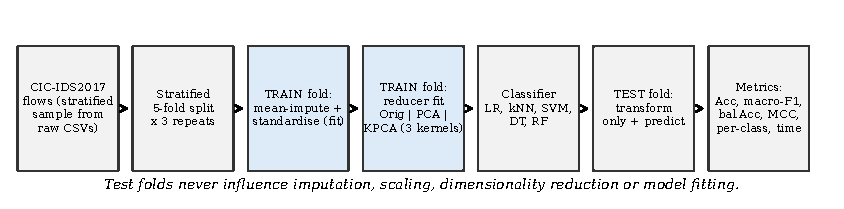
\includegraphics[width=\textwidth]{fig1_pipeline.pdf}
\caption{Experimental pipeline. All data-dependent preprocessing and reduction is fitted on the training fold only.}\label{fig:pipe}
\end{figure*}

\textbf{Classifiers.} Logistic regression (L2, lbfgs), $k$-NN with $k=5$ \cite{cover1967}, an SVM with RBF kernel, $C=1$ and $\gamma$=``scale'' \cite{cortes1995}, a decision tree with entropy criterion \cite{quinlan1986}, and a random forest with 100 trees \cite{breiman2001}, using scikit-learn \cite{pedregosa2011}. The main grid uses these fixed default settings; a separate nested search (below) tests whether tuning changes the conclusions. Each classifier except $k$-NN is also run with \texttt{class\_weight=balanced}. A majority-class classifier is the trivial baseline. Resampling (e.g.\ SMOTE) is not used: Heartbleed has only 8--9 training records per fold, too few for meaningful synthetic interpolation.

\textbf{Validation.} Repeated stratified 5-fold cross-validation, 3 repeats (15 folds), seed 42; every method sees identical folds, giving paired observations. Test folds hold about 2 Heartbleed and 4 SQL-injection records, so per-class estimates for these classes are noisy; we report means and standard deviations over the 15 folds.

\textbf{Nested cross-validation for selection.} Choosing the best of 189 configurations (21 feature spaces $\times$ 9 classifier/weighting variants) on the folds that also produce the reported score is optimistic. We therefore evaluate selection on the \emph{same} 15 outer folds: inside each outer training set (4{,}800 records), a stratified 3-fold inner cross-validation scores every configuration by macro-F1, the best is selected, and only that configuration is scored on the untouched outer test fold. We apply it to (A) the global selection and, per classifier, to (C) the best \emph{reduced} space and weighting versus (D) the original space with the weighting chosen the same way. Reducers, scalers and classifiers are refitted on every inner training split.

\textbf{Nested hyper-parameter search.} For $k$-NN, SVM and random forest on four spaces (original, PCA-30, KPCA-cosine-30, KPCA-RBF-30), a 3-fold inner cross-validation inside each of the first five outer folds selects from small grids: $k\in\{3,5,7,11\}$; SVM $C\in\{0.1,1,10\}$, $\gamma\in\{\text{scale},0.01,0.1\}$, class weight none/balanced; random forest 100/200 trees, depth none/10/20, class weight none/balanced. The RBF width of the KPCA reducer itself is not tuned.

\textbf{Row-order robustness checks (proxy chronology).} The raw files have no timestamps. Row order within each file is strongly structured (attack flows occur in contiguous blocks), so we \emph{assume} that row order follows capture time; this is not proven. (i) \emph{Head/tail split}: the first 70\,\% of each file's rows train, the last 30\,\% test. (ii) \emph{Blocked CV}: each file is cut into five contiguous blocks and each block position is held out in turn. Because every attack family occurs on a single day, whole-day splits would leave test classes unseen, so only classes present in both training and test are scored (macro-F1 over those classes; the number scored is reported). A random split of the same rows, scored on the same classes, is the comparator, so the row-order penalty is measured on identical class sets.

\textbf{Metrics.} Accuracy; macro-precision, macro-recall and macro-F1; weighted-F1; balanced accuracy; and the multi-class Matthews correlation coefficient (MCC) as implemented in scikit-learn (Chicco and Jurman argue for MCC in the binary case \cite{chicco2020}). \textbf{Macro-F1 is the primary model-selection criterion}, chosen before the runs because it weights all 15 classes equally. Per-class results and the confusion matrix use pooled out-of-fold predictions of the first repeat.

\textbf{Statistics.} For each classifier we compare feature spaces at a matched $n=10$ with two-sided Wilcoxon signed-rank tests on the 15 paired macro-F1 values, Holm-corrected over the 30 comparisons, with the matched-pairs rank-biserial correlation $r$ as effect size, and Friedman omnibus tests, following the non-parametric procedures discussed by Dem\v{s}ar \cite{demsar2006} (written for comparisons over multiple data sets; here the blocks are cross-validation folds of a single sample). Because cross-validation folds share training data, the 15 differences are positively correlated and naive $p$-values are too liberal (optimistic) \cite{nadeau2003}; Nadeau and Bengio derive a corrected variance for random subsampling, which we do not apply here; we use them for screening, not as proof. The comparisons of the original space with each classifier's \emph{best} reduced space are selected on the same folds, which favours the reduced space; the nested analysis removes that bias.

\textbf{Cost.} A serial benchmark (no parallel workers) records training and inference time (median of 5 repetitions, one fold split) and peak memory from Python's \texttt{tracemalloc}, measured in a separate pass. Native allocations inside compiled code are not traced, so memory figures are lower bounds most reliable for comparing reducers.

\section{Experimental Setup}
All experiments ran on a 2-vCPU Intel Xeon @ 2.10\,GHz virtual machine with 7\,GB RAM (Linux, Python 3.13, scikit-learn 1.9, NumPy 2.5, SciPy 1.18). The main grid contains 21 feature spaces $\times$ 9 classifier/weighting variants $\times$ 15 folds plus the baseline (2{,}850 fits) and took about 28 minutes with two workers; the nested cross-validation took about 64 minutes and the tuning search about 16 minutes. Timings in Table~\ref{tab:rt} come from the separate serial benchmark at 4{,}800 training and 1{,}200 test records. A further run repeats five spaces at $n=10$ with 10 random stratified splits at training sizes 2{,}400, 3{,}600 and 4{,}800.

\section{Results}
\subsection{Original-feature baseline and the cost of reading accuracy alone}
Predicting the majority class gives accuracy 0.672 but macro-F1 0.054 and MCC 0.000. The random forest on original features reaches accuracy $0.972\pm0.004$ but macro-F1 $0.901\pm0.020$ (weighted-F1 0.971, balanced accuracy 0.883, MCC $0.948\pm0.008$): accuracy exceeds macro-F1 by 0.071, and the gap comes from a few classes. Per class (Table~\ref{tab:perclass}), ten of the 15 classes, including benign, DDoS, the four DoS families, both Patator brute-force classes, PortScan and Heartbleed, have F1 $\ge$ 0.96. The weak points are web brute force (F1 0.53) and web XSS (0.59), which are largely mistaken for each other (48 of 103 brute-force records are predicted as XSS and 35 of 101 XSS records as brute force; Fig.~\ref{fig:cm}), then bot (0.87; recall 0.82), infiltration (0.875; recall 0.78, 36 records) and SQL injection (0.84; 21 records). Engelen et al.\ find that most web brute-force and XSS flows carry no payload in the forward direction \cite{engelen2021}, which may explain why they are hard to separate. These are the weak points that accuracy hides (Fig.~\ref{fig:acc}).

\begin{table}[t]
\caption{Per-class results of the selected model (RF, original features), pooled out-of-fold predictions, first repeat.}\label{tab:perclass}
\centering\tabsize
\begin{tabular}{lrrrr}
\toprule
Class & Precision & Recall & F1 & Support \\
\midrule
BENIGN & 0.984 & 0.996 & 0.990 & 4034 \\
Bot & 0.924 & 0.817 & 0.867 & 104 \\
DDoS & 0.997 & 0.997 & 0.997 & 340 \\
DoS GoldenEye & 0.975 & 0.966 & 0.970 & 119 \\
DoS Hulk & 0.998 & 0.979 & 0.988 & 424 \\
DoS Slowhttptest & 0.955 & 0.973 & 0.964 & 110 \\
DoS slowloris & 1.000 & 0.927 & 0.962 & 110 \\
FTP-Patator & 1.000 & 1.000 & 1.000 & 111 \\
Heartbleed & 1.000 & 1.000 & 1.000 & 11 \\
Infiltration & 1.000 & 0.778 & 0.875 & 36 \\
PortScan & 0.989 & 0.981 & 0.985 & 270 \\
SSH-Patator & 1.000 & 0.943 & 0.971 & 106 \\
Web Brute Force & 0.581 & 0.485 & 0.529 & 103 \\
Web Sql Injection & 0.941 & 0.762 & 0.842 & 21 \\
Web XSS & 0.558 & 0.624 & 0.589 & 101 \\
\bottomrule
\end{tabular}

\end{table}

\begin{figure}[t]\centering
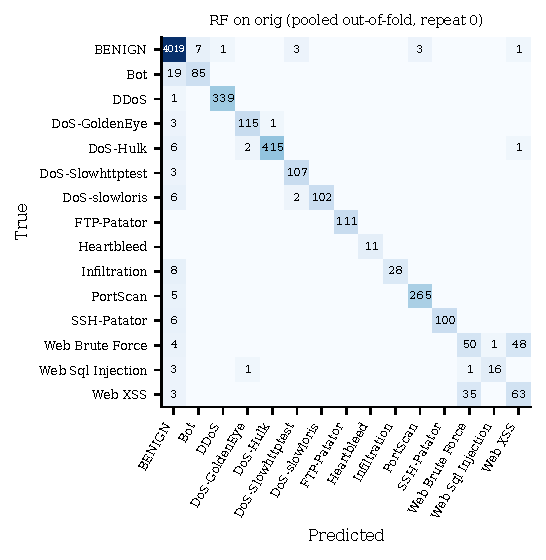
\includegraphics[width=0.85\columnwidth]{fig8_confusion_best.pdf}
\caption{Confusion matrix of RF on original features (pooled out-of-fold predictions, first repeat; colour scale compressed).}\label{fig:cm}
\end{figure}

\begin{figure*}[t]\centering
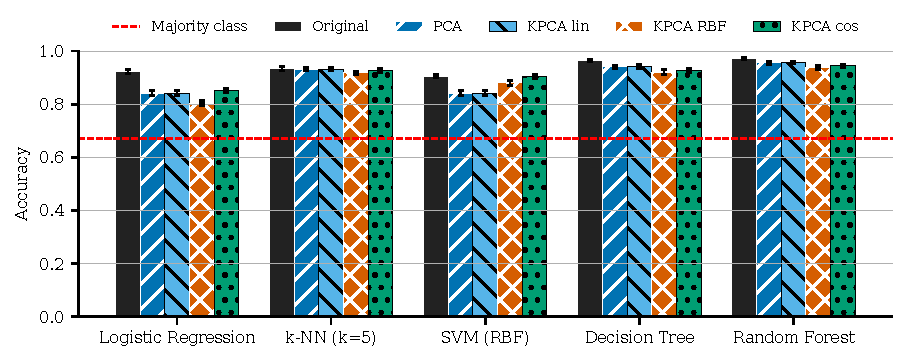
\includegraphics[width=\textwidth]{fig3_accuracy.pdf}\\[2pt]
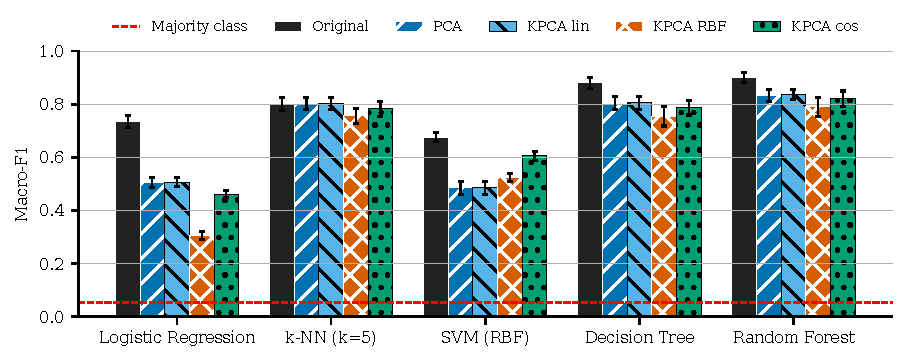
\includegraphics[width=\textwidth]{fig4_macro_f1.pdf}
\caption{Accuracy (top) and macro-F1 (bottom), mean $\pm$ std over 15 folds, 10 components for reduced spaces, standard class weights. Dashed line: majority-class classifier. Axes start at zero.}\label{fig:acc}\label{fig:f1}
\end{figure*}

\subsection{Original space versus PCA versus Kernel PCA}
Table~\ref{tab:n10} and Fig.~\ref{fig:f1} compare spaces at $n=10$. Of the 30 Holm-corrected comparisons, 23 were significant. The original space was significantly better than PCA-10 for logistic regression, SVM, decision tree and random forest, and than RBF-10 and cosine-10 for all five classifiers; for $k$-NN it was indistinguishable from PCA-10 ($\Delta$ macro-F1 $-0.001$). Among the reduced spaces, RBF-KPCA was significantly worse than PCA for LR, $k$-NN, DT and RF, but \emph{better} than PCA for the SVM; cosine KPCA was significantly better than PCA for the SVM ($+0.120$), worse for LR, $k$-NN and DT, and not different for RF. Linear KPCA and PCA did not differ significantly for any classifier. The Friedman omnibus tests (spaces at $n=10$ within each classifier; classifiers within each space) were all significant (statistics 46.8--57.6 and 51.9--58.1, Holm-adjusted $p\le 2.7\times10^{-9}$ in every case), but they inherit the fold-dependence caveat above and serve only as screening. Against each classifier's \emph{best} reduced space (Table~\ref{tab:best}), original features were clearly better for DT ($+0.070$) and RF ($+0.056$; $p_\mathrm{Holm}=0.0003$, better in all 15 folds); for logistic regression the best reduced space (PCA, 30 components) came within 0.004 ($p_\mathrm{Holm}=0.021$, a significant but negligible gap); $k$-NN showed no difference; and the SVM was the single clear case where reduction helped: cosine KPCA with 30 components raised macro-F1 from 0.675 to 0.746 ($p_\mathrm{Holm}=0.0003$, better in all 15 folds). That family of comparisons is selected on the same folds and therefore optimistic. The SVM gain also depends on component count: at 10 components, cosine KPCA is still below the original space (0.605 vs 0.675), and the SVM benefits from more components (cosine KPCA: 0.520, 0.605, 0.690, 0.725, 0.746 for 5--30 components).

\begin{table*}[t]
\caption{Accuracy / macro-F1 ($\pm$ std over 15 folds) at 10 components (original = 78 features), standard class weights.}\label{tab:n10}
\centering\tabsize
\resizebox{\textwidth}{!}{\begin{tabular}{lccccc}
\toprule
Space & LR & KNN & SVM & DT & RF \\
\midrule
Original (78) & 0.924 / 0.736$\pm$0.022 & 0.934 / 0.800$\pm$0.024 & 0.906 / 0.675$\pm$0.017 & 0.964 / 0.881$\pm$0.021 & 0.972 / 0.901$\pm$0.020 \\
PCA-10 & 0.842 / 0.506$\pm$0.018 & 0.932 / 0.802$\pm$0.023 & 0.842 / 0.485$\pm$0.024 & 0.941 / 0.805$\pm$0.025 & 0.956 / 0.834$\pm$0.022 \\
KPCA-lin-10 & 0.842 / 0.507$\pm$0.017 & 0.932 / 0.802$\pm$0.023 & 0.842 / 0.485$\pm$0.024 & 0.942 / 0.806$\pm$0.024 & 0.957 / 0.836$\pm$0.019 \\
KPCA-RBF-10 & 0.805 / 0.306$\pm$0.015 & 0.918 / 0.757$\pm$0.029 & 0.880 / 0.525$\pm$0.016 & 0.920 / 0.755$\pm$0.037 & 0.937 / 0.790$\pm$0.037 \\
KPCA-cos-10 & 0.852 / 0.462$\pm$0.012 & 0.926 / 0.783$\pm$0.028 & 0.904 / 0.605$\pm$0.018 & 0.928 / 0.786$\pm$0.027 & 0.944 / 0.821$\pm$0.029 \\
\bottomrule
\end{tabular}
}
\end{table*}

\begin{table}[t]
\caption{Original features versus each classifier's best reduced space (Wilcoxon, Holm-corrected). Positive $\Delta$: original better.}\label{tab:best}
\centering\tabsize
\resizebox{\columnwidth}{!}{\begin{tabular}{llrrrrr}
\toprule
Clf & Best reduced space & F1 orig & F1 reduced & $\Delta$F1 (orig-red.) & $p_{Holm}$ & $r$ \\
\midrule
LR & pca-30 & 0.736 & 0.731 & 0.004 & 0.021 & 0.733 \\
KNN & kpca-linear-10 & 0.800 & 0.802 & -0.001 & 1.000 & 0.000 \\
SVM & kpca-cosine-30 & 0.675 & 0.746 & -0.070 & 0.000 & -1.000 \\
DT & pca-15 & 0.881 & 0.811 & 0.070 & 0.000 & 1.000 \\
RF & pca-30 & 0.901 & 0.845 & 0.056 & 0.000 & 1.000 \\
\bottomrule
\end{tabular}
}
\end{table}

\subsection{Selection optimism: nested cross-validation}\label{sec:results-nested}
Selecting the best of 189 configurations on the scoring folds is optimistic, so we repeated the selection inside a nested cross-validation (Section~\ref{sec:method}). The configuration chosen on inner folds reached macro-F1 $0.900\pm0.022$ (accuracy 0.972, MCC 0.947) on the outer folds, against 0.901 for the same-CV maximum: an optimism of about 0.001, negligible here, because one configuration stands well above the rest. The inner cross-validation chose an original-feature configuration in all 15 outer folds (random forest 11 times, decision tree with standard or balanced weights 3 and 1 times). Table~\ref{tab:nested} compares, per classifier, the original space with the best reduced space and weighting chosen in the inner folds. Original features were clearly better for DT ($+0.093$) and RF ($+0.062$), practically equal for logistic regression ($+0.004$) and $k$-NN ($+0.002$), and worse for the SVM ($-0.060$: the inner folds chose cosine KPCA with 30 components in all 15 outer folds). The logistic-regression gap is statistically detectable (unadjusted $p=0.010$) but 0.004 is far below the fold standard deviation of 0.022. The $p$-values are unadjusted paired Wilcoxon tests over 15 outer folds that share training data.

\begin{table}[t]
\caption{Nested-CV macro-F1 ($\pm$ std over 15 outer folds): original features with the class weighting chosen on inner folds (D) versus the best reduced space and weighting chosen on inner folds (C). $\Delta=$ D$-$C; $p$: unadjusted paired Wilcoxon.}\label{tab:nested}
\centering\tabsize
\resizebox{\columnwidth}{!}{\begin{tabular}{lcccc}
\hline
Classifier & Original (D) & Reduced, chosen (C) & $\Delta$ (D$-$C) & $p$ \\
\hline
Logistic Regression & 0.736$\pm$0.022 & 0.731$\pm$0.022 & +0.004 & 0.010 \\
k-NN (k=5) & 0.800$\pm$0.024 & 0.799$\pm$0.022 & +0.002 & 0.107 \\
SVM (RBF) & 0.686$\pm$0.019 & 0.746$\pm$0.014 & $-$0.060 & $<$0.001 \\
Decision Tree & 0.891$\pm$0.023 & 0.799$\pm$0.031 & +0.093 & $<$0.001 \\
Random Forest & 0.901$\pm$0.020 & 0.839$\pm$0.024 & +0.062 & $<$0.001 \\
\hline
\end{tabular}
}
\end{table}

\subsection{Effect of hyper-parameter tuning}
Table~\ref{tab:tuning} reports the nested search (five outer folds). Tuning left the random forest unchanged (original 0.901 default, 0.899 tuned; best reduced 0.842 vs 0.839), so the ranking for tree ensembles does not depend on defaults. For $k$-NN, tuning gave $+0.007$ on original features. Under default settings the best reduced space was cosine KPCA-30 (0.801, a gap of 0.000); after tuning it was PCA-30 (0.810 versus 0.808 for the original space, a gap of $-0.002$); measured in the tuned-best space (PCA-30) the default gap is $+0.003$. In every case the $k$-NN difference is far below fold-to-fold variation. The SVM changed most: tuned macro-F1 rose from 0.668 to 0.791 on original features and from 0.745 to 0.812 with cosine KPCA-30, so the reduced-space advantage shrank from 0.076 to 0.021, with cosine KPCA at least as good as the original space in four of five folds. Five folds cannot establish a 0.021 difference, and the selected values sit on grid edges (SVM $C=10$ in all 20 selections, $k$-NN $k=3$ in all 20), so a wider grid might move the result further. We therefore treat the SVM advantage of KPCA as a property of the default RBF-SVM that largely disappears with tuning, not as a robust benefit of KPCA.

\begin{table*}[t]
\caption{Nested hyper-parameter search: mean macro-F1 over five outer folds. For each setting (default, tuned) the best reduced space among PCA-30, KPCA-cos-30 and KPCA-RBF-30 is chosen by that setting\textquoteright s own score; $\Delta$ = original $-$ reduced (negative: reduction better). K-cos-30 = KPCA, cosine kernel, 30 components. The last column gives the default-setting gap measured in the tuned-best reduced space.}\label{tab:tuning}
\centering\tabsize
\resizebox{\textwidth}{!}{\begin{tabular}{lccrrccrrr}
\toprule
 & \multicolumn{4}{c}{Default settings} & \multicolumn{4}{c}{Tuned (nested search)} & \\
\cmidrule(lr){2-5}\cmidrule(lr){6-9}
Classifier & Orig. & Best red. space & Red. & $\Delta$ & Orig.  & Best red. space  & Red.  & $\Delta$  & $\Delta$ def. at tuned-best space \\
\midrule
KNN & 0.801 & KPCA-cos-30 & 0.801 & 0.000 & 0.808 & PCA-30 & 0.810 & -0.002 & 0.003 \\
SVM & 0.668 & KPCA-cos-30 & 0.745 & -0.076 & 0.791 & KPCA-cos-30 & 0.812 & -0.021 & -0.076 \\
RF & 0.901 & PCA-30 & 0.842 & 0.059 & 0.899 & PCA-30 & 0.839 & 0.060 & 0.059 \\
\bottomrule
\end{tabular}
}
\end{table*}

\subsection{Row-order robustness (proxy chronology)}
In the head/tail split the training part has 4{,}199 records and the test part 1{,}769 scored records (32 test records of classes absent from training were dropped); only seven of the 15 classes occur in both parts (benign, bot, DDoS, DoS GoldenEye, infiltration, PortScan, SSH-Patator), and infiltration has only four test records. Table~\ref{tab:temporal} shows macro-F1 over these classes. Under the head/tail split the random forest on original features scored 0.838 versus 0.948 for a random split of the same rows and classes, and the decision tree 0.846 versus 0.959, a penalty of about 0.11. Reduced spaces suffered at least as much: RF on PCA-10 0.759 and on cosine KPCA-30 0.704, so the ordering of the original space above the reduced ones for DT, RF and LR was preserved. $k$-NN remained a near tie (original 0.790, cosine KPCA-30 0.806), and the SVM again favoured cosine KPCA-30 (0.616 vs 0.479) with default settings. In the blocked cross-validation (Table~\ref{tab:blocked}; 6, 9, 10, 8 and 6 classes scored in the five folds) the random forest scored 0.851 on original features versus 0.932 for random folds on the same classes, and the original space again led PCA-10 and cosine KPCA-30 for DT, RF and LR (RF 0.807 and 0.812); $k$-NN spaces were within 0.02, and cosine KPCA-30 again led the SVM (0.662 vs 0.581). These checks rest on the assumption that row order follows capture time, score only a subset of classes, and use single splits or five folds, so they support the ranking but give no precise penalty.

\begin{table}[t]
\caption{Head/tail (row-order) within-file split vs random split of the same rows (macro-F1 over the seven classes present in both parts). Penalty = random $-$ head/tail.}\label{tab:temporal}
\centering\tabsize
\resizebox{\columnwidth}{!}{\begin{tabular}{llrrr}
\toprule
Classifier & Space & Random & Chronological & Penalty \\
\midrule
LR & Original (78) & 0.827 & 0.687 & 0.140 \\
LR & PCA-10 & 0.653 & 0.408 & 0.245 \\
LR & KPCA-cos-30 & 0.679 & 0.508 & 0.171 \\
KNN & Original (78) & 0.860 & 0.790 & 0.070 \\
KNN & PCA-10 & 0.861 & 0.758 & 0.102 \\
KNN & KPCA-cos-30 & 0.872 & 0.806 & 0.065 \\
SVM & Original (78) & 0.715 & 0.479 & 0.236 \\
SVM & PCA-10 & 0.549 & 0.442 & 0.107 \\
SVM & KPCA-cos-30 & 0.856 & 0.616 & 0.240 \\
DT & Original (78) & 0.959 & 0.846 & 0.113 \\
DT & PCA-10 & 0.873 & 0.708 & 0.165 \\
DT & KPCA-cos-30 & 0.869 & 0.691 & 0.178 \\
RF & Original (78) & 0.948 & 0.838 & 0.111 \\
RF & PCA-10 & 0.904 & 0.759 & 0.145 \\
RF & KPCA-cos-30 & 0.915 & 0.704 & 0.211 \\
\bottomrule
\end{tabular}
}
\end{table}

\begin{table}[t]
\caption{Blocked (contiguous-in-row-order) 5-fold CV vs random 5-fold on the same classes (macro-F1 over classes present in both train and test per fold; mean over folds).}\label{tab:blocked}
\centering\tabsize
\resizebox{\columnwidth}{!}{\begin{tabular}{llrrr}
\toprule
Classifier & Space & Random & Blocked & Penalty \\
\midrule
LR & Original (78) & 0.795 & 0.677 & 0.118 \\
LR & PCA-10 & 0.551 & 0.424 & 0.126 \\
LR & KPCA-cos-30 & 0.683 & 0.533 & 0.150 \\
KNN & Original (78) & 0.864 & 0.764 & 0.100 \\
KNN & PCA-10 & 0.860 & 0.771 & 0.089 \\
KNN & KPCA-cos-30 & 0.870 & 0.783 & 0.087 \\
SVM & Original (78) & 0.723 & 0.581 & 0.142 \\
SVM & PCA-10 & 0.523 & 0.405 & 0.117 \\
SVM & KPCA-cos-30 & 0.818 & 0.662 & 0.156 \\
DT & Original (78) & 0.917 & 0.858 & 0.059 \\
DT & PCA-10 & 0.862 & 0.795 & 0.067 \\
DT & KPCA-cos-30 & 0.861 & 0.783 & 0.077 \\
RF & Original (78) & 0.932 & 0.851 & 0.081 \\
RF & PCA-10 & 0.892 & 0.807 & 0.085 \\
RF & KPCA-cos-30 & 0.893 & 0.812 & 0.081 \\
\bottomrule
\end{tabular}
}
\end{table}

\subsection{Kernel and component count}
Linear KPCA is mathematically equivalent to PCA on centred data. The two were identical for $k$-NN and SVM and within 0.001 for logistic regression; for the tree models the macro-F1 differences were small (decision tree $\le0.004$ and random forest $\le0.005$ at standard weights; $\le0.007$ and $\le0.005$ over all weightings), which we attribute to small numerical differences between eigen-solvers changing split choices (not tested). Hence a result obtained with a random forest on ``linear KPCA, 10 components'' is a PCA result, not evidence for a nonlinear kernel. Component count mattered more than kernel for logistic regression (macro-F1 0.37 at 5 PCA components to 0.73 at 30, versus 0.736 on the original features) and for the SVM; for $k$-NN, DT and RF the kernel moved macro-F1 slightly more than the component count, with both effects small (Fig.~\ref{fig:comp}). RBF-KPCA with the default $\gamma$ was the weakest kernel for LR, $k$-NN, DT and RF. For the SVM, cosine KPCA was the best kernel (macro-F1 averaged over component counts 0.657, versus 0.536 for linear and 0.515 for RBF), although RBF beat PCA at 10 components (0.525 vs 0.485). We did not tune $\gamma$, so this is a statement about the default.

\begin{figure*}[t]\centering
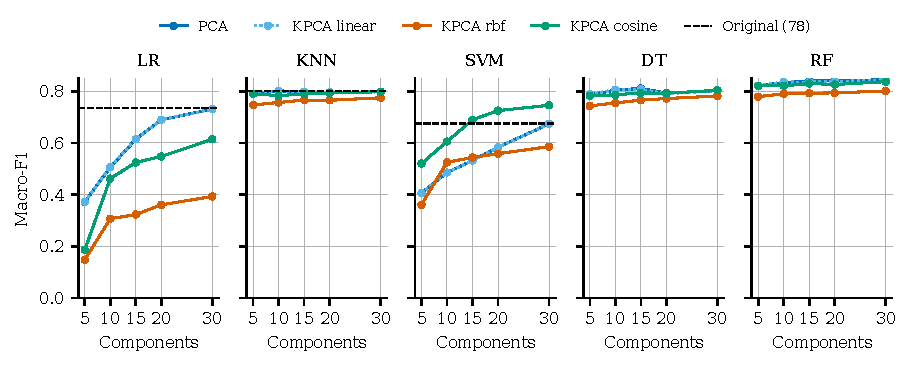
\includegraphics[width=\textwidth]{fig6_components_vs_f1.pdf}
\caption{Macro-F1 versus number of components for PCA and three KPCA kernels; dashed line: original 78 features.}\label{fig:comp}
\end{figure*}

\subsection{Class weighting}
Balanced class weights raised balanced accuracy for LR (0.748 $\to$ 0.863) and SVM (0.680 $\to$ 0.827) on the original features, but macro-F1 rose only for SVM (0.675 $\to$ 0.686) and DT (0.881 $\to$ 0.892) and \emph{fell} for LR (0.736 $\to$ 0.710) and RF (0.901 $\to$ 0.885). The best macro-F1 overall nonetheless remained the unweighted random forest, so the selected model does not depend on this choice.

\subsection{Computational cost}
Table~\ref{tab:rt} summarises the serial benchmark at 4{,}800 training / 1{,}200 test records. KPCA fitting took 5.5--5.6\,s against 0.02\,s for PCA, increased decision-tree training time from 0.07\,s (PCA) to 5.3--5.6\,s and random-forest training from 0.84--0.90\,s to 6.3--6.6\,s, and multiplied random-forest inference time by roughly five (0.020--0.021\,s to 0.092--0.123\,s per 1{,}200 records), since each new sample needs kernel evaluations against all training records. Peak traced memory was 363\,MB for KPCA against 9.8\,MB for PCA or no reduction. Over $n=400,800,1600,3200,4800$ the traced peak memory of KPCA grew roughly quadratically (3.1, 11.0, 41.6, 161.3, 359.1\,MB; log--log slope 1.9 between $n=800$ and $4800$), consistent with $n\times n$ float64 kernel matrices (184\,MB at $n=4800$, so the traced peak is about twice one matrix); single-run fit times grew faster still (0.08\,s to 5.9\,s, slope 2.4). As a purely \emph{theoretical order-of-magnitude estimate} (not a measurement and not a tested requirement), one dense float64 kernel matrix for all 2{,}830{,}743 source flows would occupy $n^2\times 8$ bytes $\approx$ 64\,TB, so exact KPCA on the full dataset would require approximation or sub-sampling (not tested here). Absolute times come from a shared 2-vCPU machine and differences below roughly a factor of two should not be over-interpreted. We make no real-time claim: only batch latencies on this machine were measured.

\begin{table}[t]
\caption{Serial runtime and traced peak memory (4{,}800 train / 1{,}200 test), median of 5.}\label{tab:rt}
\centering\tabsize
\resizebox{\columnwidth}{!}{\begin{tabular}{lrrrrr}
\toprule
Space & Reducer fit (s) & DT train (s) & RF train (s) & RF infer. (s) & Peak mem (MB) \\
\midrule
Original (78) & 0.000 & 0.113 & 0.838 & 0.020 & 9.817 \\
PCA-10 & 0.025 & 0.068 & 0.901 & 0.021 & 9.751 \\
KPCA-lin-10 & 5.466 & 5.321 & 6.251 & 0.092 & 363.434 \\
KPCA-RBF-10 & 5.594 & 5.455 & 6.644 & 0.123 & 363.434 \\
KPCA-cos-10 & 5.468 & 5.612 & 6.446 & 0.104 & 363.434 \\
\bottomrule
\end{tabular}
}
\end{table}

\subsection{Sensitivity to training-set size}
Fig.~\ref{fig:size} shows macro-F1 at 2{,}400, 3{,}600 and 4{,}800 training records over 10 random splits each. For LR, DT and RF the original space had the highest mean macro-F1 at every size, and for the SVM at 3{,}600 and 4{,}800 (at 2{,}400, cosine KPCA was 0.009 higher); for $k$-NN the spaces overlap within one standard deviation. This is a stability check within the same sample and distribution, not a test of generalization to unseen traffic.

\begin{figure*}[t]\centering
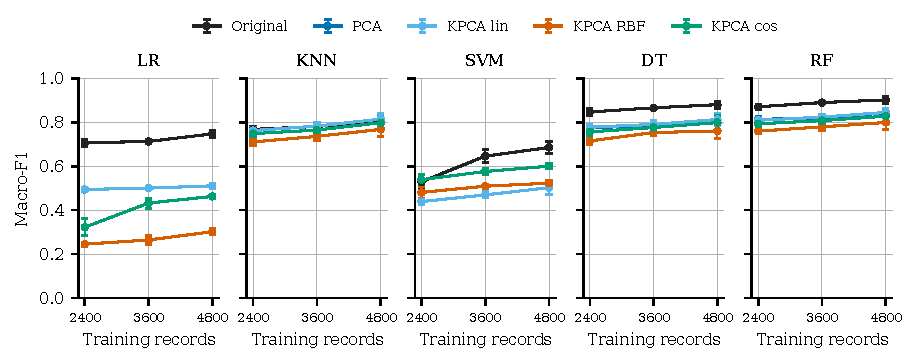
\includegraphics[width=\textwidth]{fig9_training_size.pdf}
\caption{Macro-F1 versus training-set size (random stratified splits, 10 per size, mean $\pm$ std); 10 components for reduced spaces.}\label{fig:size}
\end{figure*}

\section{Discussion}
\textbf{Answers to the research questions.} RQ1/RQ2: on this sample, reducing 78 standardised features to 5--30 PCA or KPCA components generally did not improve and usually lowered macro-F1: clearly for decision tree and random forest, negligibly or not at all for logistic regression (at 30 components) and $k$-NN, and the one gain, for the RBF-SVM with cosine KPCA, largely disappeared under tuning (0.076 to 0.021). RQ3: for $k$-NN, DT and RF the kernel moved macro-F1 slightly more than component count, whereas for LR and SVM component count mattered more; RBF (default $\gamma$) was weakest for four of five classifiers, and linear KPCA equals PCA. RQ4: KPCA multiplied reducer fitting time by more than 200 and traced memory by about 37 at $n=4{,}800$ and scales quadratically in memory, with no accuracy benefit for four of five classifiers. RQ5: orderings were stable across repeated folds, training sizes, nested selection, tuning of three classifiers, and (as far as they can be scored) head/tail and blocked row-order splits.

\textbf{Why accuracy misleads.} The benign class makes up 67.2\,\% of records, so the trivial baseline already has accuracy 0.672. The best model's accuracy of 0.972 corresponds to macro-F1 0.901, and its web-attack F1 values are 0.53 and 0.59. The gap is smaller than in a preliminary 1{,}000-record experiment that is not reported here, but still conceals a systematic failure on two classes. Weighted-F1 and accuracy from a single split can neither reveal this nor show whether a difference of a point or two is noise (fold standard deviations of macro-F1 are 0.02).

\textbf{Plausible but untested explanations.} Tree ensembles are insensitive to monotone feature scaling and can exploit individual informative features; projecting onto a few leading components may discard low-variance but discriminative directions. Heavy-tailed flow features also make variance-based reduction and the default RBF width poorly matched. These are hypotheses we did not test (e.g.\ with tuned $\gamma$, robust scaling, or supervised reduction).

\section{Threats to Validity and Limitations}
These limitations are real, and the conclusions should be read as conditional on them.

\textbf{1. Sample, not full data.} All results come from \emph{one} stratified sample of 6{,}000 records out of 2.5\,M de-duplicated flows (0.24\,\%), because exact KPCA is quadratic in memory. The sample is class-stratified with a floor of 100 records per class, \emph{not} prevalence-preserving: attack classes are over-represented relative to real traffic, so accuracy, macro-F1 and class priors do not describe deployment-time prevalence. Heartbleed (11 records), SQL injection (21) and infiltration (36) are complete but tiny, so their per-class estimates are very uncertain, and a different random sample could change rankings that differ by a few points. We did not repeat the whole pipeline over several sampling seeds.

\textbf{2. Leakage status.} Sampling was performed on the raw, un-imputed data, and imputation, scaling and reduction are fitted inside each training fold. Remaining possible leakage channels were \emph{not} eliminated: records from the same attack session or burst can still fall into both training and test folds in the random 5-fold design, and near-duplicate (not exact-duplicate) flows are not removed. The row-order checks reduce but do not remove this concern, and they rest on the unproven assumption that row order follows capture time.

\textbf{3. Limited external validity.} All data come from one dataset captured in one testbed over one week. The row-order checks score only seven classes (head/tail split) or six to ten classes per fold (blocked) and use a single split or five folds; there is no cross-dataset evaluation (cross-evaluation is discussed in \cite{apruzzese2022}; evaluation pitfalls in \cite{arp2022}). The conclusions apply to random and within-file row-ordered splits of CIC-IDS2017 only; they say nothing about true temporal drift.

\textbf{4. Selection and inference.} The headline configuration (RF, original features) was the best of 189 on the same cross-validation that produced its score. The nested analysis shows the optimism is about 0.001 macro-F1 here, but the nested estimate itself is conditioned on the same sample. Repeated-CV significance tests violate independence \cite{nadeau2003}; $p$-values are screening evidence, and unadjusted values are reported for the nested comparisons.

\textbf{5. Limited tuning.} Hyper-parameter search covered only $k$-NN, SVM and random forest, four spaces and five outer folds, with small grids whose optimum lay on the edge for $k$-NN and SVM $C$. Logistic regression, the decision tree and the KPCA kernel parameters ($\gamma$ for RBF) were not tuned, so conclusions about those are about default settings. Class weighting was the only imbalance treatment; resampling was not evaluated.

\textbf{6. Dataset quality.} The original CIC-IDS2017 flows contain known labelling and feature-construction artefacts \cite{engelen2021}, which may inflate or distort scores (and may be why web brute force and XSS are confused); we did not use the corrected release.

\textbf{7. Cost measurements.} Timings and memory come from one 2-vCPU virtual machine, memory is a traced Python/NumPy lower bound, and the 64\,TB figure is arithmetic ($n^2\times8$ bytes), not a measurement. No approximate KPCA method was tested.

This study proposes no new algorithm, and we make no claim of state-of-the-art, real-time, production-ready or generalizable performance. The supported finding is narrower: on this sample, original features were at least as good as PCA or KPCA for four of five classifiers, the one exception largely vanished with tuning, and accuracy hid a systematic failure on web attacks.

\section{Conclusion}
On a 6{,}000-record sample drawn, after exact same-label duplicate removal, from all eight CIC-IDS2017 daily files and under repeated cross-validation with fold-wise fitting of imputation, scaling and reduction, a random forest on the original 78 features had the highest observed macro-F1 among the evaluated configurations (macro-F1 $0.901\pm0.020$, accuracy $0.972\pm0.004$; $0.900\pm0.022$ when the selection itself is nested). PCA and Kernel PCA with 5--30 components generally did not improve on the original features: they were clearly worse for decision tree and random forest, practically equal for logistic regression (at 30 components) and $k$-NN, and helped mainly the RBF-SVM (cosine KPCA, 30 components), an advantage that shrank from 0.076 to 0.021 once a small hyper-parameter grid was tuned. The ranking survived the head/tail and blocked row-order splits (macro-F1 lower by 0.06--0.25 on the classes that could be scored), although these rest on an assumed row order. Linear KPCA coincided with PCA, so a gain reported for linear-kernel KPCA is a gain of PCA. KPCA cost more than 200 times more reducer-fit time and 37 times more traced memory at 4{,}800 records, growing roughly quadratically. Accuracy (0.972) concealed weak and mutually confused detection of web brute force and XSS (F1 0.53, 0.59). The results are limited to this sample and to CIC-IDS2017.

\textbf{Future work.} Repeat the pipeline over several sampling seeds and larger samples with an approximate KPCA; add cross-dataset evaluation; widen the tuning grids and tune the KPCA kernel parameters; test the corrected CIC-IDS2017 release \cite{engelen2021}; and evaluate session-grouped splits.


\section*{Data and Code Availability}
The raw CIC-IDS2017 MachineLearningCVE files are distributed by the dataset provider \cite{sharafaldin2018} and are not redistributed here. The sampling script, the sampling manifest (file names, raw and de-duplicated class counts, seed), all experiment, analysis and claim-checking code, per-fold raw results and the generated tables and figures are available at [REPOSITORY URL / ARCHIVE DOI - TO BE FILLED BY THE AUTHORS]; the file \texttt{RUN\_EXPERIMENTS.md} lists the commands. The main grid takes about 30 minutes on two cores and the nested cross-validation about one hour.

\section*{Acknowledgment}
\textbf{AI-assistance disclosure.} Generative AI was used in this work, and it is disclosed here in accordance with IEEE policy. The AI system was Claude (Anthropic; Claude Code with the Claude Sonnet 5.5 model, and Claude subagents for citation checking). It was used for: (i) writing and revising the Python code of the experimental pipeline (data preparation, cross-validation, nested cross-validation, hyper-parameter search, row-order checks, statistical tests, runtime benchmark, and the generation of tables and figures from the result files) and an automated script that compares the numbers in this article with the result files; (ii) drafting and editing the text of all sections of this article, including the abstract, captions and limitations; and (iii) retrieving bibliographic metadata and cross-checking statements attributed to cited sources. The level of use was substantial for code and for drafting and editing the text. All reported numbers were produced by code run on the data described and re-checked by script. [THE AUTHORS MUST CONFIRM THAT THIS STATEMENT IS ACCURATE AND COMPLETE BEFORE SUBMISSION.] The authors reviewed the content and remain fully responsible for it.

\begin{thebibliography}{17}
\bibitem{ring2019} M. Ring, S. Wunderlich, D. Scheuring, D. Landes, and A. Hotho, ``A survey of network-based intrusion detection data sets,'' \textit{Comput. Secur.}, vol. 86, pp. 147--167, Sep. 2019, doi:10.1016/j.cose.2019.06.005.

\bibitem{sharafaldin2018} I. Sharafaldin, A. H. Lashkari, and A. A. Ghorbani, ``Toward generating a new intrusion detection dataset and intrusion traffic characterization,'' in \textit{Proc. 4th Int. Conf. Inf. Syst. Security and Privacy (ICISSP)}, 2018, pp. 108--116.

\bibitem{engelen2021} G. Engelen, V. Rimmer, and W. Joosen, ``Troubleshooting an intrusion detection dataset: the CICIDS2017 case study,'' in \textit{Proc. IEEE Security and Privacy Workshops (SPW)}, 2021, pp. 7--12, doi:10.1109/SPW53761.2021.00009.

\bibitem{panigrahi2018} R. Panigrahi and S. Borah, ``A detailed analysis of CICIDS2017 dataset for designing intrusion detection systems,'' \textit{Int. J. Eng. Technol.}, vol. 7, no. 3.24, pp. 479--482, 2018.

\bibitem{arp2022} D. Arp \textit{et al.}, ``Dos and don'ts of machine learning in computer security,'' in \textit{Proc. 31st USENIX Security Symp.}, 2022, pp. 3971--3988.

\bibitem{abdulhammed2019} R. Abdulhammed, H. Musafer, A. Alessa, M. Faezipour, and A. Abuzneid, ``Features dimensionality reduction approaches for machine learning based network intrusion detection,'' \textit{Electronics}, vol. 8, no. 3, Art. no. 322, 2019.

\bibitem{scholkopf1998} B. Sch\"olkopf, A. Smola, and K.-R. M\"uller, ``Nonlinear component analysis as a kernel eigenvalue problem,'' \textit{Neural Comput.}, vol. 10, no. 5, pp. 1299--1319, 1998.

\bibitem{kuang2014} F. Kuang, W. Xu, and S. Zhang, ``A novel hybrid KPCA and SVM with GA model for intrusion detection,'' \textit{Appl. Soft Comput.}, vol. 18, pp. 178--184, 2014.

\bibitem{apruzzese2022} G. Apruzzese, L. Pajola, and M. Conti, ``The cross-evaluation of machine learning-based network intrusion detection systems,'' \textit{IEEE Trans. Netw. Service Manag.}, vol. 19, no. 4, pp. 5152--5169, Dec. 2022, doi:10.1109/TNSM.2022.3157344.

\bibitem{pedregosa2011} F. Pedregosa \textit{et al.}, ``Scikit-learn: Machine learning in Python,'' \textit{J. Mach. Learn. Res.}, vol. 12, pp. 2825--2830, 2011.

\bibitem{cortes1995} C. Cortes and V. Vapnik, ``Support-vector networks,'' \textit{Mach. Learn.}, vol. 20, no. 3, pp. 273--297, 1995.

\bibitem{cover1967} T. Cover and P. Hart, ``Nearest neighbor pattern classification,'' \textit{IEEE Trans. Inf. Theory}, vol. 13, no. 1, pp. 21--27, 1967.

\bibitem{quinlan1986} J. R. Quinlan, ``Induction of decision trees,'' \textit{Mach. Learn.}, vol. 1, no. 1, pp. 81--106, 1986.

\bibitem{breiman2001} L. Breiman, ``Random forests,'' \textit{Mach. Learn.}, vol. 45, no. 1, pp. 5--32, 2001.

\bibitem{chicco2020} D. Chicco and G. Jurman, ``The advantages of the Matthews correlation coefficient (MCC) over F1 score and accuracy in binary classification evaluation,'' \textit{BMC Genomics}, vol. 21, Art. no. 6, 2020.

\bibitem{demsar2006} J. Dem\v{s}ar, ``Statistical comparisons of classifiers over multiple data sets,'' \textit{J. Mach. Learn. Res.}, vol. 7, pp. 1--30, 2006.

\bibitem{nadeau2003} C. Nadeau and Y. Bengio, ``Inference for the generalization error,'' \textit{Mach. Learn.}, vol. 52, no. 3, pp. 239--281, 2003.
\end{thebibliography}

\begin{IEEEbiographynophoto}{[AUTHOR NAME 1 - TO BE FILLED]}
[BIOGRAPHY - TO BE FILLED BY THE AUTHOR: degrees, institutions and years; current position; research interests.]
\end{IEEEbiographynophoto}

\begin{IEEEbiographynophoto}{[AUTHOR NAME 2 - TO BE FILLED]}
[BIOGRAPHY - TO BE FILLED BY THE AUTHOR.]
\end{IEEEbiographynophoto}

\EOD
\end{document}
